\documentclass[ignoreframetext]{beamer}
\usepackage[utf8]{inputenc}
\usepackage[T1]{fontenc}
\usepackage[british]{babel}
\usepackage{booktabs}

\usepackage[all]{foreign}
\renewcommand{\foreignfullfont}{}
\renewcommand{\foreignabbrfont}{}

\usepackage{newclude}
\usepackage{import}

\usepackage[strict]{csquotes}
\usepackage[single]{acro}

\usepackage[natbib,style=alphabetic,maxbibnames=99]{biblatex}
\addbibresource{slides.bib}

\usepackage{subcaption}

\usepackage[noend]{algpseudocode}
\usepackage{xparse}

\let\email\texttt

\usepackage{listings}
\lstset{%
  basicstyle=\footnotesize,
  numbers=left
}

\usepackage{amsmath}
\usepackage{amssymb}
\usepackage{mathtools}
\usepackage{amsthm}
\usepackage{thmtools}
\usepackage[unq]{unique}
\DeclareMathOperator{\powerset}{\mathcal{P}}

\usepackage[binary-units]{siunitx}

\usepackage[capitalize]{cleveref}

\usetheme{Berlin}
\setbeamertemplate{footline}%{miniframes theme}
{%
  \begin{beamercolorbox}[colsep=1.5pt]{upper separation line foot}
  \end{beamercolorbox}
  \begin{beamercolorbox}[ht=2.5ex,dp=1.125ex,%
    leftskip=.3cm,rightskip=.3cm plus1fil]{author in head/foot}%
    \leavevmode{\usebeamerfont{author in head/foot}\insertshortauthor}%
    \hfill%
    {\usebeamerfont{institute in head/foot}\usebeamercolor[fg]{institute in head/foot}\insertshortinstitute}%
  \end{beamercolorbox}%
  \begin{beamercolorbox}[ht=2.5ex,dp=1.125ex,%
    leftskip=.3cm,rightskip=.3cm plus1fil]{title in head/foot}%
    {\usebeamerfont{title in head/foot}\insertshorttitle} \hfill     \insertframenumber%
  \end{beamercolorbox}%
  \begin{beamercolorbox}[colsep=1.5pt]{lower separation line foot}
  \end{beamercolorbox}
}
\setbeamercovered{transparent}
\setbeamertemplate{bibliography item}[text]

\AtBeginSection[]{%
  \begin{frame}<beamer>
    \tableofcontents[currentsection]
  \end{frame}
}

\ProvideDocumentEnvironment{assumption}{o}{%
  \IfValueTF{#1}{%
    \begin{block}{Assumption: #1}
  }{%
    \begin{block}{Assumption}
  }
}{%
  \end{block}
}

\ProvideDocumentEnvironment{protocol}{o}{%
  \IfValueTF{#1}{%
    \begin{block}{Protocol: #1}
  }{%
    \begin{block}{Protocol}
  }
}{%
  \end{block}
}

\ProvideDocumentEnvironment{remark}{o}{%
  \IfValueTF{#1}{%
    \begin{alertblock}{Note: #1}
  }{%
    \begin{alertblock}{Note}
  }
}{%
  \end{alertblock}
}

\ProvideDocumentEnvironment{idea}{o}{%
  \IfValueTF{#1}{%
    \begin{block}{Idea: #1}
  }{%
    \begin{block}{Idea}
  }
}{%
  \end{block}
}

\ProvideDocumentEnvironment{question}{o}{%
  \setbeamercolor{block body}{bg=orange!15,fg=black}
  \setbeamercolor{block title}{bg=orange,fg=white}
  \setbeamercolor{local structure}{fg=orange}
  \IfValueTF{#1}{%
    \begin{block}{Question: #1}
  }{%
    \begin{block}{Question}
  }
}{%
  \end{block}
}

\ProvideDocumentEnvironment{exercise}{o}{%
  \setbeamercolor{block body}{bg=yellow!10,fg=black}
  \setbeamercolor{block title}{bg=yellow,fg=black}
  \setbeamercolor{local structure}{fg=yellow}
  \IfValueTF{#1}{%
    \begin{block}{Exercise: #1}
  }{%
    \begin{block}{Exercise}
  }
}{%
  \end{block}
}


\begin{document}
\mode<all>
\mode*

\section{Programming by CLI}

\begin{frame}[fragile]
  \begin{solution}[Most important]
    \begin{itemize}
      \item GUI is a User Interface (UI).
      \item The API is an interface for writing programs.
      \item CLI is a hybrid; it's a UI, but it can easily be used to write 
        programs.
    \end{itemize}
  \end{solution}

  \begin{example}[Counting the number of files]
    \begin{minted}{bash}
ls | wc -l
    \end{minted}
  \end{example}
\end{frame}

\begin{frame}
  \begin{figure}
    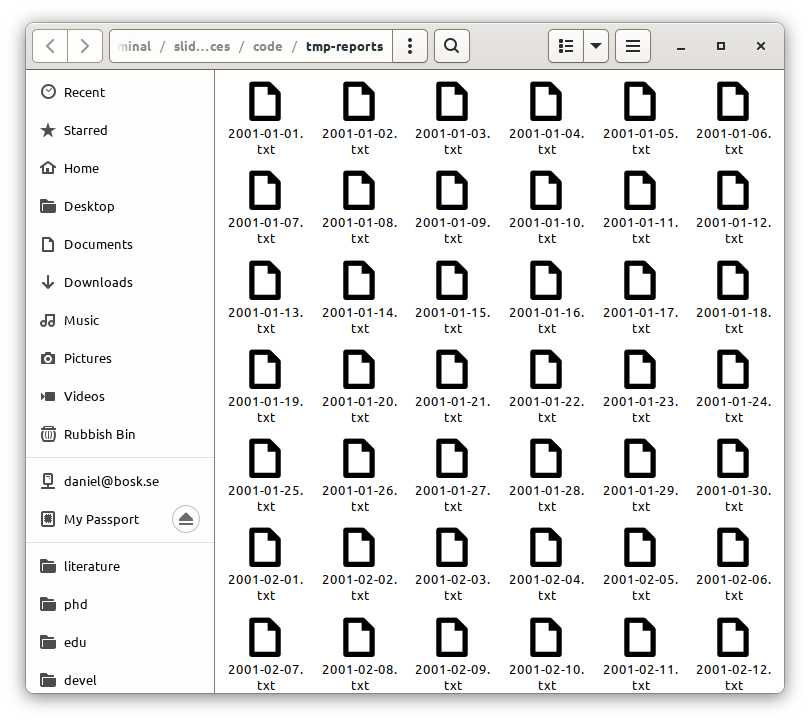
\includegraphics[height=0.5\textheight]{fig/many-reports.png}
    \caption{file explorer showing many dated report files.}
  \end{figure}

  \begin{exercise}[Printing contents of specific files]
    \begin{itemize}
      \item Take the contents of all reports from summers of 2005--2008.
      \item Put into one file.
    \end{itemize}
  \end{exercise}
\end{frame}

\begin{frame}[fragile]
  \begin{figure}
    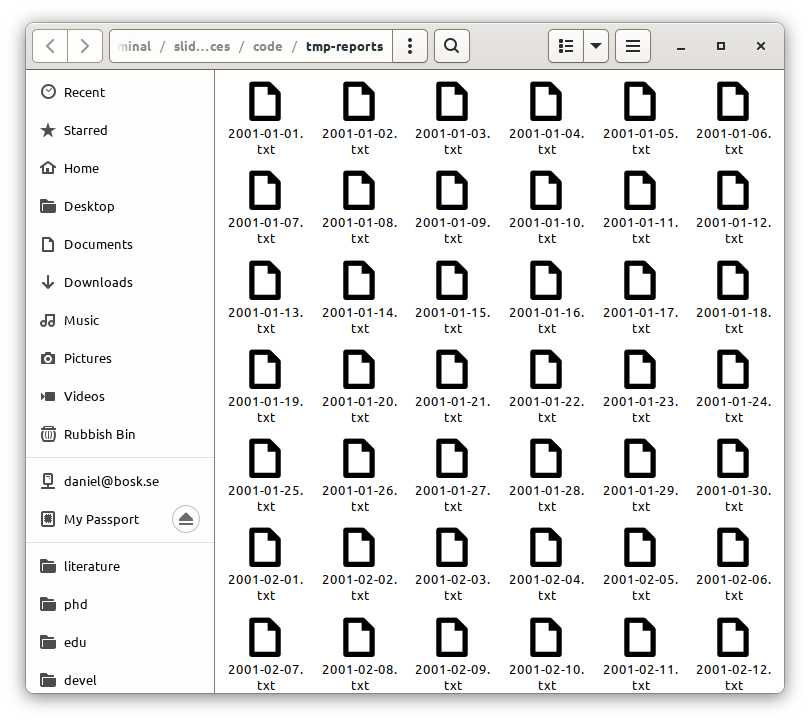
\includegraphics[height=0.5\textheight]{fig/many-reports.png}
    \caption{file explorer showing many dated report files.}
  \end{figure}

  \begin{solution}[CLI-solution: \texttt{summer.sh}]
    \inputminted[firstline=3]{bash}{code/summer.sh}
  \end{solution}
\end{frame}


\section{Scripting}

\begin{frame}
  \begin{figure}
    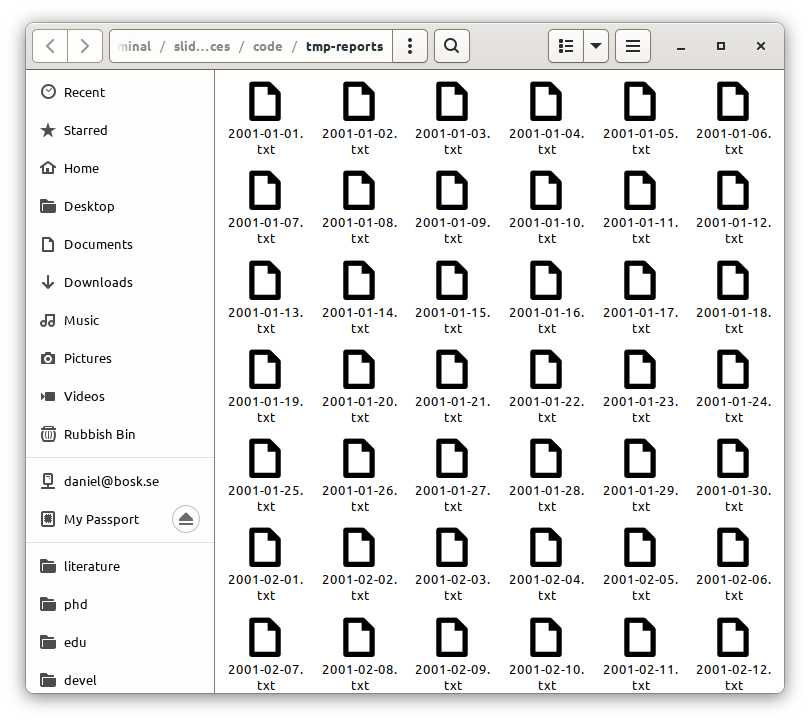
\includegraphics[height=0.5\textheight]{fig/many-reports.png}
    \caption{file explorer showing many dated report files.}
  \end{figure}

  \begin{exercise}
    \begin{enumerate}
      \item Sort the reports into subdirectories, one directory per year.
      \item For each year, sort the reports into the subdirectories: summer, 
        autumn, winter and spring.
    \end{enumerate}
  \end{exercise}
\end{frame}

\begin{frame}[fragile]
  \begin{example}[Positional arguments, \texttt{args.sh}]
    \begin{itemize}
      \item \texttt{args.sh:}
    \end{itemize}
    \inputminted[linenos,highlightlines={2,3}]{bash}{code/args.sh}
    \begin{itemize}
      \item \texttt{bash args.sh one two three}
    \end{itemize}
    \begin{minted}[highlightlines={2,3}]{text}
fixed: one two three
order: one two three
unorder: three two one
    \end{minted}
  \end{example}
\end{frame}

\begin{frame}[fragile]
  \begin{example}[\texttt{vars.sh:}]
    \inputminted[linenos,firstline=3,highlightlines={5,6}]{bash}{code/vars.sh}
  \end{example}
\end{frame}

\begin{frame}[fragile]
  \begin{solution}[Sorting the reports]
    \inputminted[linenos,firstline=3,lastline=11,highlightlines=3]{bash}{code/sort.sh}
  \end{solution}
\end{frame}

\begin{frame}
  \begin{remark}
    \begin{itemize}
      \item The grading scripts are written like this.
    \end{itemize}
  \end{remark}

  \begin{example}[Grading terminal assignment]
    \inputminted[linenos,firstline=55,lastline=70,fontsize=\scriptsize]{bash}{code/grade.sh}
  \end{example}
\end{frame}

\mode*
\end{document}
